Peg Solitaire er et spil hvor en person skal forsøge at fjerne pinde i
et bræt med huller ved at foretage en række træk indtil der kun er en
pind tilbage på brættet. I hvert træk kan en pind fjernes ved at en
nabopind flyttes over pinden til et ledigt hul. For hvert træk
efterlades brættet med en pind færre.

\begin{minipage}{.8\linewidth}
I den klassiske engelske version af spillet Peg Solitaire består
brættet af 33 huller, som til at starte med er fyldt med 32 pinde; det
midterste hul i brættet er ikke udfyldt og opgaven består i at det
netop er det midterste hul, der til slut skal indeholde en pind.
\end{minipage}
\begin{minipage}{.2\linewidth}
  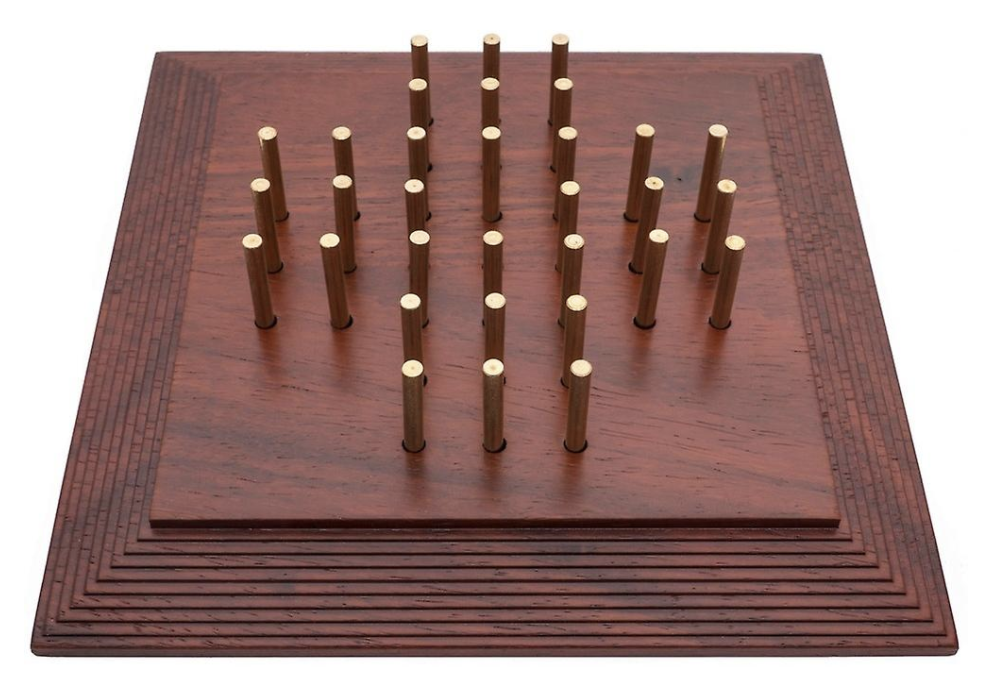
\includegraphics[width=\linewidth]{solitaire.png}
\end{minipage}

I denne opgave skal der arbejdes mod at få computeren til at finde en
løsning til den engelske version af Peg Solitaire. En løsning vil
bestå i at computeren udskriver de træk der skal flyttes. Opgaven er
delt i tre dele. I den første delopgave arbejdes der mod at
implementere et modul til at repræsentere en brætkonstellation samt
operationer til at foretage flytninger og derved danne nye
brætkonstellationer. I den anden delopgave skal der arbejdes mod at
gøre det muligt for en spiller at spille spillet ved brug
af \texttt{fsharpi} således at computeren tillader at der foretages træk
hvorefter den nye brætkonstellation udskrives. I den tredie delopgave skal
der skrives en algoritme, som returnerer en liste af træk, der
efterlader en enkelt pind i midten af brættet.
